\subsection {Collection}
\label{sec:Collection}
The \sbol{Collection} class is a class that groups together a set of \sbol{TopLevel} objects that have something in common.
Some examples of \sbol{Collection} objects:
\begin{itemize}
\item Results of a query to find all \sbol{Component} objects in a repository that function as promoters.
\item A set of \sbol{Component} objects representing a library of genetic logic gates.
\item A \sbol{Component} for a complex design, and all of the \sbol{Component}, \sbol{Component},\\ \sbol{Sequence}, and \sbol{Model} objects used to provide its full specification.
\end{itemize}

\begin{figure}[ht]
\begin{center}
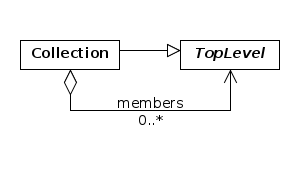
\includegraphics[scale=0.6]{uml/collection}
\caption[]{Diagram of the \sbol{Collection} class and its associated properties.}
\label{uml:collection}
\end{center}
\end{figure}

\subparagraph{The \sbolheading{members} property}\label{sec:members}
The \sbol{members} property of a \sbol{Collection} is OPTIONAL and MAY contain a set of \sbol{URI} references to zero or more \sbol{TopLevel} objects.

\subsubsection{Namespace}
\label{sec:Namespace}
The \sbol{Namespace} class is a subclass of \sbol{Collection} and is used to define \sbol{member} entities that share the same prefix in their \sbol{identity} properties. All linked objects must have a URI prefix matching the identity of a \sbol{Namespace} object. 

\begin{figure}[ht]
\begin{center}
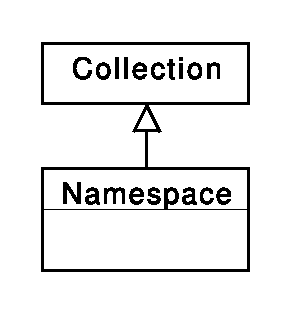
\includegraphics[scale=0.6]{uml/namespace}
\caption[]{\sbol{Namespace} is a special case of \sbol{Collection}.}
\label{uml:namespace}
\end{center}
\end{figure}

\subsubsection{Experiment}
\label{sec:Experiment}


\begin{figure}[ht]
\begin{center}
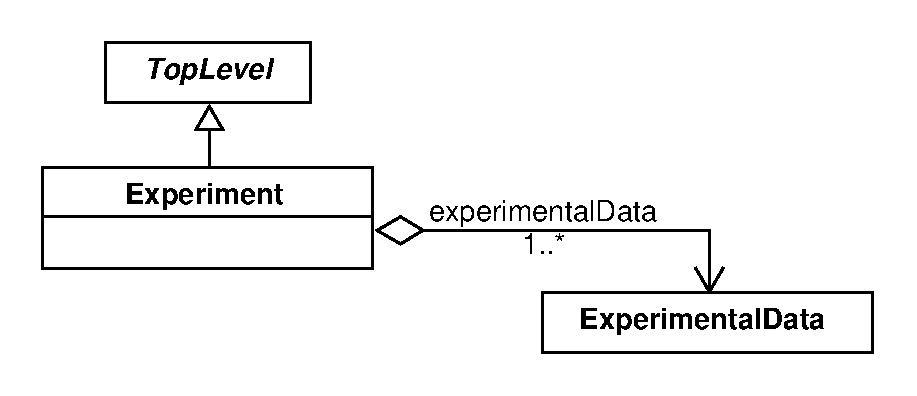
\includegraphics[scale=0.6]{uml/experiment}
\caption[]{Diagram of the \sbol{Experiment} class and its associated properties.}
\label{uml:experiment}
\end{center}
\end{figure}

The purpose of the \sbol{Experiment} class is to aggregate experimental data sets for subsequent analysis, usually in accordance with an experimental design. 

As shown in \ref{uml:experimental_data}, the \sbol{Experiment} class aggregates \sbol{ExperimentalData} objects via the \sbol{experimentalData} property.

\subparagraph{ The \sbolheading{experimentalData} property}\label{sec:experimentalData}
The \sbol{experimentalData} property is OPTIONAL and MAY contain a set of \sbol{URI} references to \sbol{ExperimentalData} objects. The same \sbol{ExperimentalData} MAY be referred to by more than one \sbol{Experiment} in this way.
